\documentclass[a4paper,14pt]{extarticle}
\usepackage{../../tex-shared/report-layout}

\renewcommand{\mylabnumber}{3}
\renewcommand{\mylabtitle}{Исследование возможностей формирования виртуальных топологий вычислительных кластеров}
\renewcommand{\mysubject}{Теория распределенных систем и параллельных вычислений}
\renewcommand{\mylecturer}{Дрозин А. Ю.}

\begin{document}
\begin{titlepage}
    
    \thispagestyle{empty}
    
    \begin{center}
        
        Министерство науки и Высшего образования Российской Федерации \\
        Севастопольский государственный университет \\
        Кафедра ИС
        
        \vfill

        Отчет \\
        по лабораторной работе №\mylabnumber \\
        \enquote{\mylabtitle} \\
        по дисциплине \\
        \enquote{\MakeTextUppercase{\mysubject}}

    \end{center}

    \vspace{1cm}

    \noindent\hspace{7.5cm} Выполнил студент группы ИС/б-17-2-о \\
    \null\hspace{7.5cm} Горбенко К. Н. \\
    \null\hspace{7.5cm} Проверил \\
    \null\hspace{7.5cm} \mylecturer

    \vfill

    \begin{center}
        Севастополь \\
        \the\year{}
    \end{center}

\end{titlepage}

\section{Цель работы}
Исследовать возможности, предоставляемые MPI по формированию виртуальных
топологий.

\section{Постановка задачи}
Вариант №1 Необходимо реализовать алгоритм перемножения матриц ленточным
способом с распределением столбцов.

\section{Ход работы}
Текст программы:
\begin{lstlisting}
#include <iostream> 
#include <mpi.h> 
#include <fstream> 
#include <iomanip> 
  
using namespace std; 
  
MPI_Comm graph; 
int processRank, processCount; 
double **aMatrix, **bMatrix, **cMatrix, *row, *column, *tmpColumn, *result; 
  
int nextProcess() { 
    int rankToNextProcess; 
    MPI_Graph_neighbors(graph, processRank, 1, &rankToNextProcess); 
    return rankToNextProcess; 
} 
  
void input(double **matrix, int n, string path) { 
    ifstream in(path); 
    for (int i = 0; i < n; i++) { 
        for (int j = 0; j < n; j++) { 
            in >> matrix[i][j]; 
        } 
    } 
} 
  
void initBuffers(double *rowsBuf, double *columnsBuf) { 
    int k = 0; 
    for (int i = 0; i < processCount; i++) { 
        for (int j = 0; j < processCount; j++) { 
            rowsBuf[k] = aMatrix[i][j]; 
            columnsBuf[k++] = bMatrix[j][i]; 
        } 
    } 
} 
  
void createGraph() { 
    int n = processCount; 
    int *index = new int[processCount]; 
    int *edges = new int[processCount]; 
    for (int i = 1; i <= processCount; i++) { 
        index[i - 1] = i; 
        edges[i - 1] = i % processCount; 
    } 
    MPI_Barrier(MPI_COMM_WORLD); 
    MPI_Graph_create(MPI_COMM_WORLD, n, index, edges, 0, &graph); 
    MPI_Comm_size(graph, &processCount); 
    MPI_Comm_rank(graph, &processRank); 
    delete[] index; 
    delete[] edges; 
} 
  
void initRowAndColumn(double *rowsBuf, double *columnsBuf, double *row, double *column) { 
    MPI_Barrier(graph); 
    MPI_Scatter(rowsBuf, processCount, MPI_DOUBLE, row, processCount, MPI_DOUBLE, 0, graph); 
    MPI_Barrier(graph); 
    MPI_Scatter(columnsBuf, processCount, MPI_DOUBLE, column, processCount, MPI_DOUBLE, 0, graph); 
} 
  
void iteration(double *row, double *column, double *result, int index) { 
    result[index] = 0; 
    for (int i = 0; i < processCount; result[index] += row[i] * column[i], i++); 
} 
  
void swapColumns(double *column, double *tmpColumn) { 
    MPI_Status status; 
    int next; 
    next = !processRank ? processCount - 1 : processRank - 1; 
    if (!(processRank % 2)) { 
        MPI_Barrier(graph); 
        MPI_Send(column, processCount, MPI_DOUBLE, next, 0, graph); 
    } 
    MPI_Barrier(graph); 
    MPI_Recv(tmpColumn, processCount, MPI_DOUBLE, nextProcess(), MPI_ANY_TAG, graph, &status); 
    if (processRank % 2) { 
        MPI_Barrier(graph); 
        MPI_Send(column, processCount, MPI_DOUBLE, next, 0, graph); 
    } 
} 
  
void mult(double *row, double *column, double *result, double *tmpColumn) { 
    int index = processRank; 
    for (int i = 0; i < processCount; i++) { 
        iteration(row, column, result, index); 
        if (i != processCount - 1) { 
            swapColumns(column, tmpColumn); 
            for (int j = 0; j < processCount; column[j] = tmpColumn[j], j++); 
        } 
        index = (index + 1) % processCount; 
    } 
} 
  
void collect() { 
    double *tmpBuf; 
    if (processRank == 0) { 
        tmpBuf = new double[processCount * processCount]; 
    } else { 
        tmpBuf = new double[1]; 
    } 
    MPI_Barrier(graph); 
    MPI_Gather(result, processCount, MPI_DOUBLE, tmpBuf, processCount, MPI_DOUBLE, 0, graph); 
    if (processRank == 0) { 
        int k = 0; 
        for (int i = 0; i < processCount; i++) { 
            for (int j = 0; j < processCount; cMatrix[i][j++] = tmpBuf[k++]); 
        } 
    } 
} 
  
void print(double **matrix) { 
    for (int i = 0; i < processCount; i++) { 
        for (int j = 0; j < processCount; cout << setw(3) << matrix[i][j++] << " "); 
        cout << endl; 
    } 
} 
  
void master() { 
    aMatrix = new double *[processCount]; 
    bMatrix = new double *[processCount]; 
    cMatrix = new double *[processCount]; 
    for (int i = 0; i < processCount; i++) { 
        aMatrix[i] = new double[processCount]; 
        bMatrix[i] = new double[processCount]; 
        cMatrix[i] = new double[processCount]; 
    } 
    input(aMatrix, processCount, "a.txt"); 
    input(bMatrix, processCount, "b.txt"); 
    result = new double[processCount]; 
    row = new double[processCount]; 
    column = new double[processCount]; 
    tmpColumn = new double[processCount]; 
    double *rowsBuf = new double[processCount * processCount]; 
    double *columnsBuf = new double[processCount * processCount]; 
    initBuffers(rowsBuf, columnsBuf); 
    initRowAndColumn(rowsBuf, columnsBuf, row, column); 
    mult(row, column, result, tmpColumn); 
    collect(); 
  
    cout << "\tA*B = C" << endl << endl; 
    print(aMatrix); 
    cout << "*" << endl; 
    print(bMatrix); 
    cout << "===============" << endl; 
    print(cMatrix); 
  
    delete aMatrix; 
    delete bMatrix; 
    delete cMatrix; 
    delete result; 
    delete row; 
    delete column; 
    delete tmpColumn; 
    delete[] rowsBuf; 
    delete[] columnsBuf; 
} 
  
void slave() { 
    result = new double[processCount]; 
    row = new double[processCount]; 
    column = new double[processCount]; 
    tmpColumn = new double[processCount]; 
    double *rowsBuf = new double[1]; 
    double *columnsBuf = new double[1]; 
    initRowAndColumn(rowsBuf, columnsBuf, row, column); 
    mult(row, column, result, tmpColumn); 
    collect(); 
    delete[] result; 
    delete[] row; 
    delete[] column; 
    delete[] tmpColumn; 
    delete[] rowsBuf; 
    delete[] columnsBuf; 
} 
  
int main(int argc, char **argv) { 
    MPI_Init(&argc, &argv); 
    MPI_Comm_rank(MPI_COMM_WORLD, &processRank); 
    MPI_Comm_size(MPI_COMM_WORLD, &processCount); 
    createGraph(); 
    processRank == 0 ? master() : slave(); 
    MPI_Finalize(); 
    return 0; 
}
\end{lstlisting}

На рисунке \ref{fig:result} представлен результат работы программы:
\begin{figure}[H]
    \centering
    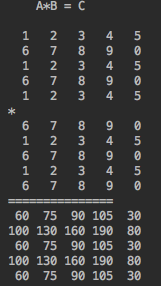
\includegraphics[width=.3\linewidth]{result}
    \caption{Результат работы программы}
    \label{fig:result}
\end{figure}

\section*{Выводы}
В ходе лабораторной работы были исследованы возможности, предоставляемые MPI по формированию виртуальных топологий.
\end{document}